\section{Server selection}
\label{sec:serverselection}

Upon a successful login, the user is presented with the main choice screen of the Jupyter Hub page as shown in Figure
\ref{fig:mainchoice}. 

\begin{figure}[!ht]
	\centering
	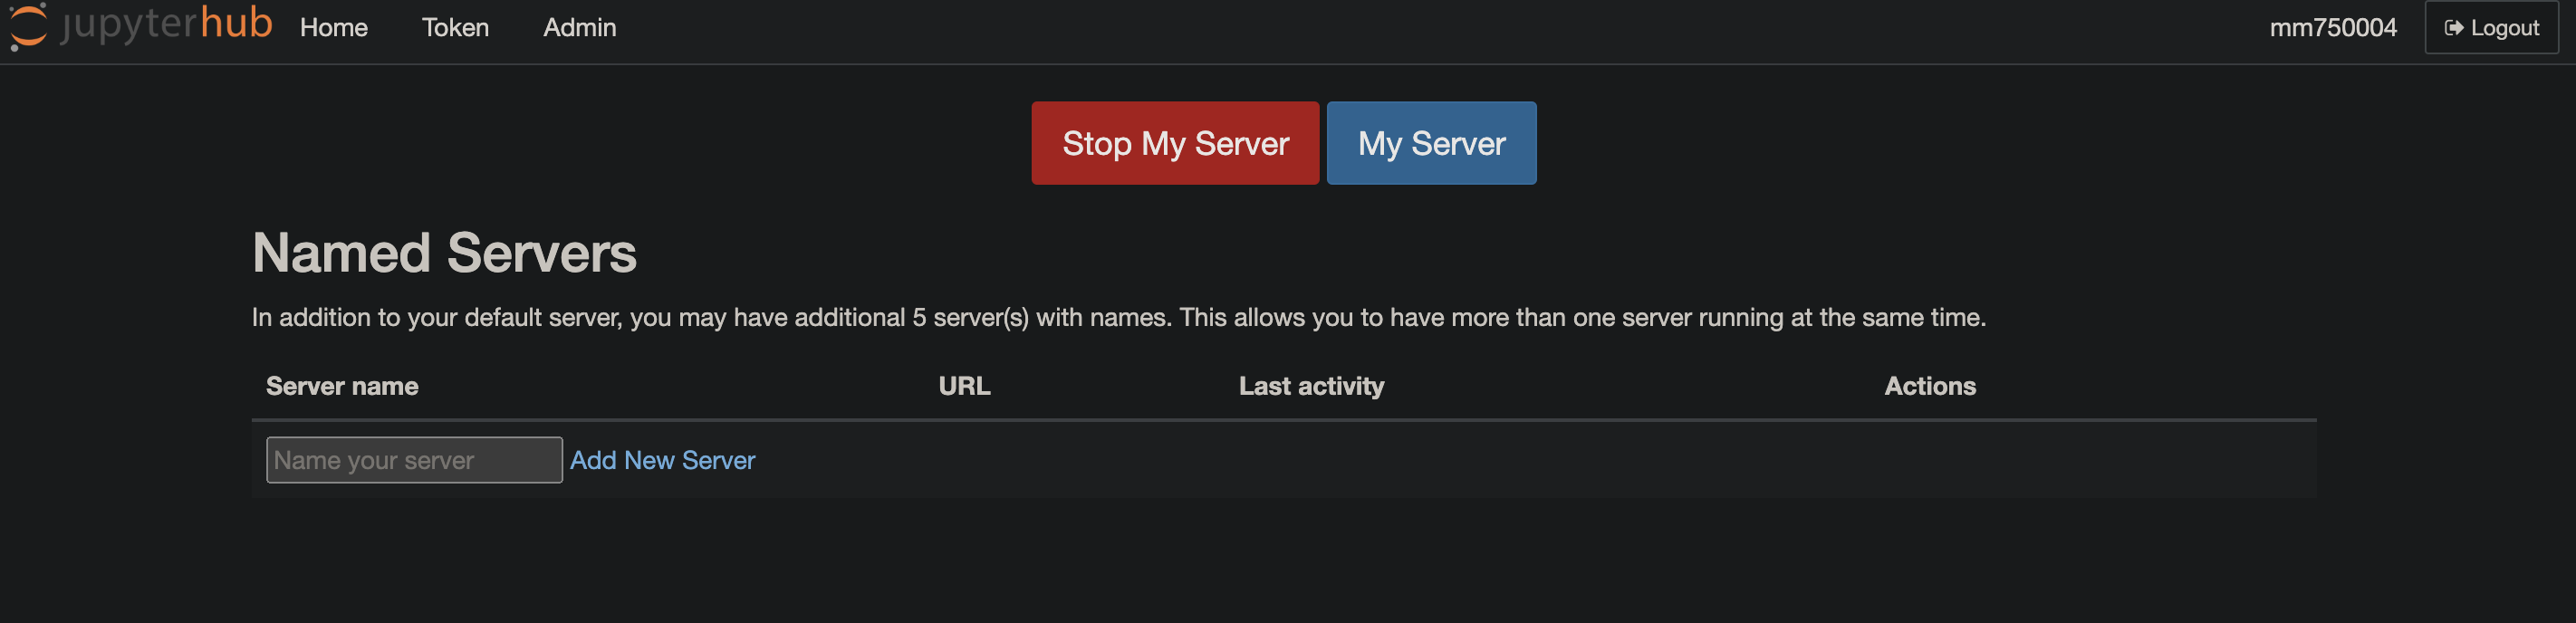
\includegraphics[width=0.7\linewidth]{img/mainchoice.png}
	\caption{Jupyter Hub main choice screen.}
	\label{fig:mainchoice}
\end{figure}

The user can manage their Jupyter servers.
The buttons on the top of the page allow the user to start a new server,
stop an existing one, or access the Jupyter Lab interface
to an already running server. The server controlled by this interface
is the main server for the user, which is named as the user name.
Additionally, the user can create up to 5 additional servers 
with different names. If figure \ref{fig:mainchoice} this is shown
as the "Named Servers" section. 


\begin{bclogo}[logo=\bcinfo, couleurBarre=orange, noborder=true, couleur=white]{Warning}
The name given to the server may only contain lowercase letters.
No special characters, uppercase letters, numbers or spaces are allowed.
\end{bclogo}

Each server is a separate instance of the Jupyter Lab interface,
each with its own storage (the home directory), image and 
allocated resources.